\documentclass{article}

\usepackage[utf8]{inputenc}
\usepackage{amsmath,physics,mathtools,listings,graphicx,pdfpages,amsfonts,amssymb,amsthm,float}

\DeclarePairedDelimiter{\opair}{\langle}{\rangle}
\newcommand\given[1][]{\:#1\vert\:}
\graphicspath{ {figures/} }
\title{The Statistics of Random Walks}
\author{Habib Rehman}
\date{June/July 2015}
\begin{document}
\maketitle

\tableofcontents

\hphantom
\newline
\section{Exposition}
This section act as an exposition to the research project.

\subsection{Aims and Objectives}
The main aims of this research project were to:
\begin{enumerate}
	\item{Identify the correspondence between the return distribution of a 1D random walk and a 2D random walk}
	\item{Consider the correspondence between the arc length distribution of a random walker returning}
\end{enumerate}
The objectives for both aims were the following:
\begin{enumerate}
	\item{Explore the physical phenomena (i.e. a stochastic process) that implicates a random walk}
	\item{Devise a mathematical model that models the physical phenomena}
	\item{Precisely delineate the properties of the mathematical model and all aspects regarding it}
	\item{Translate the mathematical model into \texttt{Python} code to implement the model}
	\item{Collect data by running the code with nuanced configurations of the mathematical model}
	\item{Analyse the data and draw conclusions to obtain results}
\end{enumerate}

\subsection{Context}
 Random walks are applied in a range of fields such as physics, financial economics, population genetics and computer science. Random walks are essential mathematical models used to model stochastic processes which are ubiquitously present in many fields. Any natural process such as diffusion is a stochastic process as it occurs randomly and is thought to be non-deterministic (unpredictable). However, modelling the process as a random walks enables us to deduce the statistics of certain behaviour of the process and thus predict the outcome (to a certain extent) to of an event which implicates the process.
The ability to predict this for stochastic processes is of great importance as it provides actionable information that can be crucial.

For instance, in finance, random walks are used to model stock prices, by considering the change of the stock prices with respect to time. Where the stock prices and the time are the independent random variables that form a 2D random walk.

In physics, random walks are essential in predicting how fast one gas will diffuse into another, how fast heat will spread in a solid, how big fluctuations in pressure will be in a small container, and many other statistical phenomena. They were used by Albert Einstein to find the size of atoms from the Brownian motion exhibited by atoms.

Additionally, in computer science, random walks are used to improve the scalability networks such as Tor \cite{dollapplications} by allowing efficient allocation of resources which prevents network latency and prevent network failure. This example has very real impacts on the users of the network as it dictates the time that they have to invest in order to receive a response to their request.

\subsection{Selection of approach}
The following are the proposed approaches initially considered out which the most effective approach was selected.

\paragraph{Approaches:}
\begin{enumerate}
	\item{Model the stock price change (with respect to time) data for a particular stock as a random walk, erase loops and then identify the correspondence between the return and arc length distributions. All implementation in \texttt{Python}}
	\item{Model the Tor network bandwidth usage (with respect to time) data as a random walk and then identify the correspondence between the return and arc length distributions. All implementation in \texttt{Python}}
	\item{Model pseudorandomly generated sequence(s) of independent variables as a random walk and then identify the correspondence between the return and arc length distributions. All implementation \texttt{C++}}
	\item{Model a pseudorandomly generated sequence(s) of independent variables as a random walk and then identify the correspondence between the return and arc length distributions. All implementation in \texttt{Python}}
\end{enumerate}

\paragraph{Selection} I selected approach 4. because it was the most practical, feasible and reproducible approach. While approach 4. doesn't use true random data like approach 1. or 2. , it does provide reproducibility as the seed used to generate pseudorandom sequence always yields the same sequence for the particular seed and thus the results can be verified by a third-party. Data obtained from approach 1. could be subject to manipulation (stock manipulation) and thus yield in unreliable results and selecting a suitable stock would pose non-problem oriented challenges. While approach 2. addresses the problems with approach 1. by definitively yield true random data \footnote{As the Tor network is fully decentralised and extensive enough in size that it is infeasible for any single entity to cause significant disturbances in the network}, it is impractical to gather the required amount of data in the time available for the research and it would also pose additional non-problem oriented challenges. Finally, approach 4. was selected over approach 3. because of its use of the \texttt{Python} programming language instead of the \texttt{C++} programming language. This is because \texttt{Python}, being a high-level language, already provided much of functionality (more extensive standard library) that we needed where as in \texttt{C++} we would have had to implement most of that needed functionality. So, \texttt{Python} enabled us to stay problem oriented and accomplish our objectives faster.

 \section{Abstract}
The purpose of this research has been to identify the precise correspondence between the return distribution of a one-dimensional random walk and a two-dimensional random walk. This research also considers the correspondence between the arc length distribution of a random walker returning and the arc length distribution of the loops erased.

\section{Introduction}
	A random walk is a stochastic process formed by the repeated summation of identically distributed (independent) random variables distributed random variables and regarded to be a is a V-valued Markov chain on a graph \cite{schweinsberg2009loop}. This research considers random walks on a integer lattice $\mathbb{Z}^\emph{{d}}$ as the discrete space, practically, allows for more analysis (operations) to be carried out with a feasible computational power. The research is also concerned with loop erased random walks in the second dimension (i.e. $d=2$) as it is below the critical dimension for random walks $d = 4$ at which the process converges to Brownian motion \cite{lawler2010} and scaling limits exist (i.e. the limit as the lattice spacing approaches zero). It becomes trivial in the regard that self-intersection becomes highly improbable. The random walks studied correspond to increment distributions with the properties of having zero mean and finite variance. These properties are necessary for normal convergence in the increments of the distributions to occur. They also allow for the succinct expression of the main result quickly. Firstly, I will delineate the statistical behaviour of a simple random walk in what follows. Thereafter, I will provide the appropriate theorems and definition for random walks and loop erased random walks.

\subsection{Simple Random Walk on a $\mathbb{Z}$ lattice.}
	The simplest non-trivial case is to let $X\textsubscript{1}, X\textsubscript{2}, \ldots, X\textsubscript{n}$ represent the outcomes of independent experiments and is in the first dimension. Suppose that these experiments are tosses of a fair coin and there is a gain of $+1$ for each head loss $-1$ on each tail. The outcome of a flip of the coin is equally likely to be heads or tails, so the walk is clearly unbiased, in that there is no preference for gain or loss. Then $S\textsubscript{n}$ represents his cumulative gain or loss on the first $n$ plays.
Then the sequence $(S\textsubscript{n})_\emph{n=0}^\infty$ would be described as a simple random walk (for this scenario its called the \emph{gambler\' s ruin estimate}) on the $\mathbb{Z}$ lattice. When the behaviour of such a simple process is analysed in detail, it becomes apparent that it more intriguing than it appears to be. What we can deduce is that:
	\begin{enumerate}
	\item The walk returns to its starting position (i.e. 0) at time $2n$ with probability
		\begin{center}
			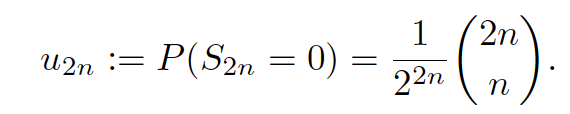
\includegraphics[scale=0.8]{WalkReturnToStartT2nProbability}
		\end{center}
		By \emph{Stirling's approximation}, it is
		\begin{center}
			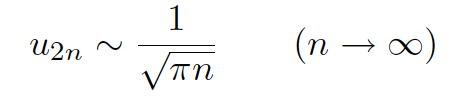
\includegraphics[scale=0.8]{WalkReturnToStartTnProbability}
			\cite{Durrett2010}
		\end{center}
	\item The walk eventually reaches each integer within $\mathbb{Z}$ lattice with certainty and so traverses it infinitely often. Suppose $S\textsubscript{0} := 0$ and $T := \inf\{n : S\textsubscript{n} = +1\}$ then $P(T < \infty) = 1$ and $P(T = \infty) = 0$
	\item The distribution of \emph{T} is
		\begin{center}
			$P(T = 2n - 1)\ =\ (-1)_{n-1}\binom{\frac{1}{2}}{n}$
		\end{center}
	\end{enumerate}
A Simple Random Walk generally refers to random walk in the first dimension. However, this research is concerned with random walks in 2 dimensions. But interestingly, a 2 dimensional random walk is essentially composed of two Simple Random Walks in either plane as the vertices in either plane selected are independently selected.
\newline


\subsection{Loop Erased Random Walks (LERW)}
	A Loop erased random walk on the integer lattice is a process obtained from Random Walk by erasing the loops chronologically. In LERW, the process is expected to have a continuum limit that is conformal, and nonrigorous conformal, field theory gives an exact prediction of the exponent as a simple rational number. In three dimensions there is no reason to believe that the exponent takes on a rational value. Once the loops are erased from the random walk, it essentially becomes a uniform spanning tree (UST), which is a spanning tree chosen uniformly at random, and so the algorithms for generating LERWs are used in application to produce uniform spanning trees.

\paragraph{Loop Erased Random Walk definition.} \label{alg:LE} If $\omega = [\omega\textsubscript{0}, \ldots, \omega\textsubscript{n}]$ is a path, then the \emph{(chronological) loop-erasure} function $LE(\omega)$ would be defined as follows\cite{klafter2011} \newline
	Let $\lambda_{0} = \max\{j\ \le \ n: \omega_{j}=0\}$.
	\newline
	Set $\beta_{0}=\omega_{0}=\omega_{\lambda_{0}}$.
	\newline
	Suppose $\lambda_{i} < n$. Let $\lambda_{i+1} = \max\{j\ \le n: \omega_{j}=\omega_{\lambda_{i}+1}\}$.
	\newline
	Set $\beta_{i+1}=\omega_{\lambda_{i+1}}=\omega_{\lambda_{i}+1}$.
	\newline
	If $i_{\omega} = \min \{i : \lambda_{i} = n\} = \min\{i : \beta_{i} = \omega_{n}\}$,

	then $LE\left(\omega\right) = \lbrack \beta_{0},\ldots,\beta_{i}\rbrack$

\section{Methodology}
	In this section, I will explain the theory behind the code that was written to produce the resultant data. The code was mainly\footnote{The \emph{raw2binned.c} script in \texttt{C++} was used for the sake of efficiency and was originally written by Francesc, later modified by Gunnar Pruessner and then adapted by me for this project} written in \texttt{Python} as it enabled us to stay problem-oriented and allowed us to implement the LERW rapidly as well as readily provided us much greater useful functionality through its extensive library. We used the Python \texttt{matplotlib} library to generate the required statistical plots from the data as it integrated seamlessly with our workflow. We also used the  \texttt{numpy} library for efficiently creating and manipulating the large matrices for the system instances.

Code distribution was a major issue as sharing code via an email did not only make it hard to keep track of it but also aroused great inconsistencies and miss communication. So, I proposed the usage of the version control systems called \emph{git}. The usage of this system enabled us to stay in sync with the latest code version of the project, resolve any conflicts in the code and update the code. So our workflow consisted simply of fetching the latest code and pushing the changes made \footnote{The changes made were committed and pushed to \emph{GitHub} (a centralised project hosting platform that uses the \emph{git} version control systems) on which the project was hosted.}, each with a single command  \footnote{In the shell/terminal/command-line}.

Overall, these changes made the tasks easier to perform and made the workflow more efficient saving us an enormous amount of time.


\subsection{Random Walk Implementation}
	The Random Walk was theoretically modelled to transverse on the 2 dimensional surface of a 3 dimensional cylinder (i.e. the system) with two vertical open boundaries and to two horizontal periodic. At the open boundaries, the Random Walk is initiated from starting boundary and ceased at the ending boundary. Due to the curvilinear geometry of a cylinder, the system had the property of allowing the random walk to transverse an infinite number of steps in any vertical direction given that the random walk did not reach the ending boundary.
The system was implemented as a 2 dimensional $\mathbb{Z}$ lattice of a particular size (length by circumference) which represented the 2 dimensional surface of the cylinder and, to implement the previously stated property of the original system, periodic boundaries where inaugurated. The function of the periodic boundaries was ensure that the random walk continues to transverse from the boundary iteratively until it took a valid step (i.e. a step within the system boundaries) when the random walk surpassed a system boundary (see Figure~\ref{fig:RW}). The following is a formal definition of the system.

\paragraph{System definition.}\label{subsec:sysfdef} Given that $\vb{S}=\opair{i, j}$ is the system of size (L, C), where \emph{i} and \emph{j} are the respective vertical and horizontal components of the system (refer to Appendix~\ref{sssec:sysdef} for the actual system definition)
	\begin{enumerate}
		\item The system generation can be expressed as
			\begin{center}
				$\vb{S} = \left\{\left. (\sum_{k=0}^L i_k, \sum_{k=0}^C j_k) \; \right\vert \;i_k j_k \in\mathbb{Z} \right\}$1
			\end{center}
		\item The length and the circumference $(L, C)$ of the system are of equal size which implies that the lattice was of equal length (for this research)
		\item $\vb{S}\textsubscript{i = 0}$ is the starting boundary and $\vb{S}\textsubscript{i = L}$, where \emph{L}  represents the length of the system, is the ending boundary.
		\item $(\vb{S}\textsubscript{i = 0}, \vb{S}\textsubscript{j = y})$  is the starting point, where \emph{y} is the first pseudorandom number in the sequence generated by lib function using a given seed.
		\item Periodic boundaries exist at $(\vb{S}\textsubscript{j = 0}, \vb{S}\textsubscript{j = C})$, where \emph{C} is the circumference of the system, to allow \emph{j} to be of an indefinite size
	\end{enumerate}

\paragraph{Random Walk generation.} A Random Walk, $S_{n}$, was generated using the generation function
	\begin{center}
		$\omega_{n} =  \sum_{k=0}^n X_k$
	\end{center}
where $\{X_k\}$ are independent and identically distributed random variables.
Implementing the periodic boundaries as well, resulted in the generation function
\begin{center}
		$\omega_{n} =  \left\{ \sum_{k=0}^n X_k \given[\Big] X_k \lnot\ (0 \lor L \lor C) \right\}$
\end{center}
I translated this into \texttt{Python} code which is viewable in Appendix~\ref{sssec:srwgen}. In the code, the \emph{trajectory} list\footnote{Collectively, the \emph{path} taken (by the random walk)} containing the running set of vertices corresponding to the pseudorandom steps that the random walk had talking was a \texttt{numpy} list because of extensive functionality (i.e functions/methods) that were required to perform the non trivial manipulations quickly as well as staying problem-oriented.

When Implementing the algorithm, I had to duplicate the trajectory list and perform some operation to it. However, the problem was that by default python only performed a so called \emph{shallow copy} of the list which is creates a new list that only references the data that the old list links to \cite{DPscopy2016}. Hence, when the new list is changed the old list is changed correspondingly as it references the same data. To resolve this issue, I made a \emph{deep copy} of the list which instead of creating a duplicate list that just references the old memory location it actually duplicates the memory location (by recursively copying the properties/methods) and creates a duplicate list with a reference to. This makes any modification to the new list independent from the old list \cite{DPscopy2016}.

While originally planned to only use \texttt{matplotlib} for plotting the analytical graphs (i.e histograms), I figured out a way to use the \texttt{matplotlib} API to plot of the actual trajectory that a random walk makes. This offered us a qualitatively insight into the structure and behaviour of a random walk with a particular system. Refer to the following figure (Figure~\ref{fig:RW}) to see a sample plot. Refer to Appendix~\ref{sssec:rwplot} for the plot code that uses the matplotlib API.
\begin{figure}[H]
	\begin{center}
		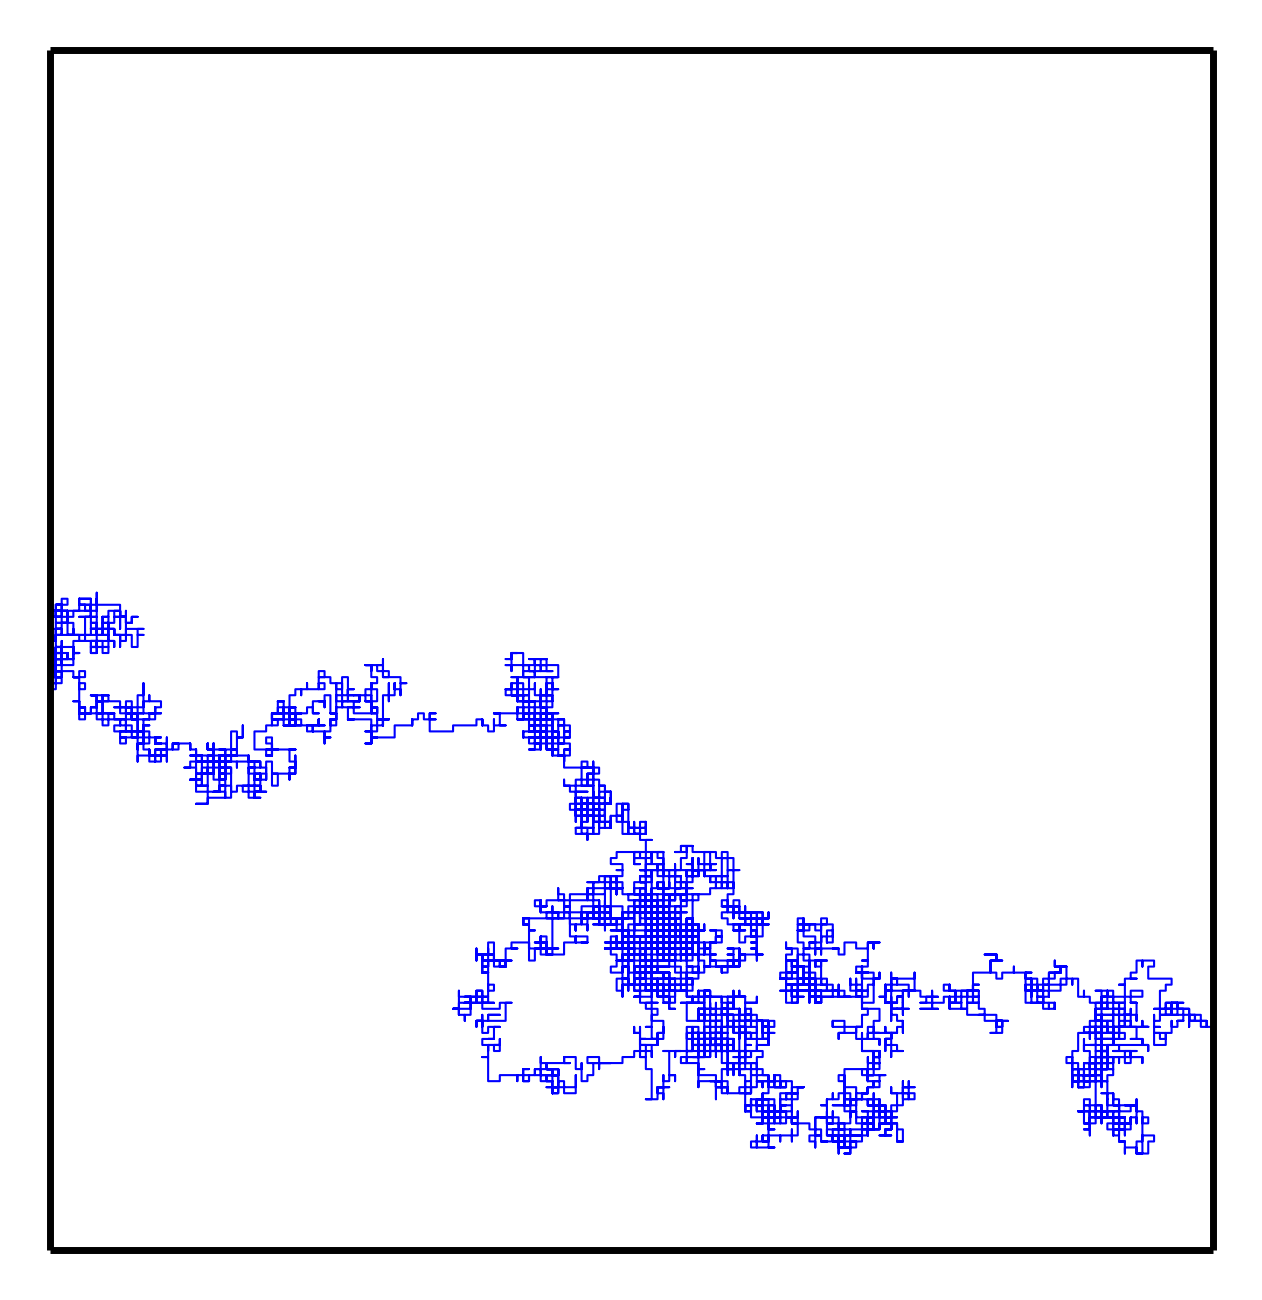
\includegraphics[scale=1.6]{RW_200s7hdpi}
		\caption{Random walk on a $\mathbb{Z}^{\emph{2}}$ lattice (system size: 200; seed: 7)}
		\label{fig:RW}
	\end{center}
\end{figure}

\paragraph{Random Walk Loop Erasure.} A loop is simply the result of the random walk intersecting itself. Considering that the random walk is transversing on an integer lattice, for a loop to occur, a vertex on the lattice has to be transversed at least twice - at the start of the loop and at the end of the loop. So to erase the loop, an algorithm was devised which removed every duplicate of a given list of vertices (i.e. the random walk trajectory) from the first occurrence of the vertex onwards to (and including) the last occurrence in the random walk trajectory list iteratively until all duplicates (i.e. loops) are removed. The $LE(\omega)$ algorithm defined in Loop Erased Random Walk definition in \S~\ref{alg:LE}, is a condensed form of the algorithm that was used to generate the LERWs to generate the data. When implementing the LERW and testing, the qualitatively insight gained from plotting the actual LERW trajectory using \texttt{matplotlib} was instrumental in evaluating the effectiveness of the code and identifying any logic errors\footnote{``A logic error (or logical error) is a mistake in a program's source code that results in incorrect or unexpected behaviour'' from $techterms.com/definition/logic\_error$}. While the \texttt{matplotlib} API sufficed for the random walk implementation, it did not achieve the expected results for the loop erased random walk because its inability to handle discontinuity that resulted from the erasure. This is evident in Figure~\ref{fig:LERWw} for the output from which we can qualitatively concluded that the output of the \texttt{matplotlib} API plot code (Appendix~\ref{sssec:rwplot}) is incorrect. So, I had to write algorithm that accounted for this by discreetly plotting the continuous sequences and then joining them. Figure~\ref{fig:LERW} is the output of the final loop erased random plot code (Appendix~\ref{sssec:lerwplot}).
Refer to Appendix~\ref{sssec:lerw} for the implementation of the LERW.

\begin{figure}[H]
	\begin{center}
		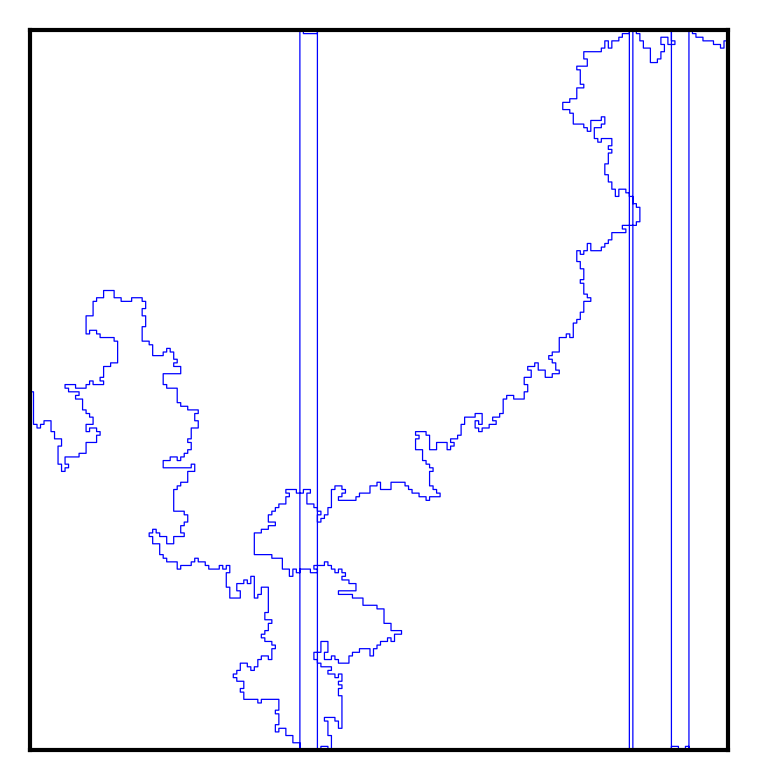
\includegraphics[scale=1.6]{LERWw}
		\caption{Loop erased random walk plot using \texttt{matplotlib} API (system size: 200; seed: 9)}
		\label{fig:LERWw}
	\end{center}
\end{figure}

\begin{figure}[H]
	\begin{center}
		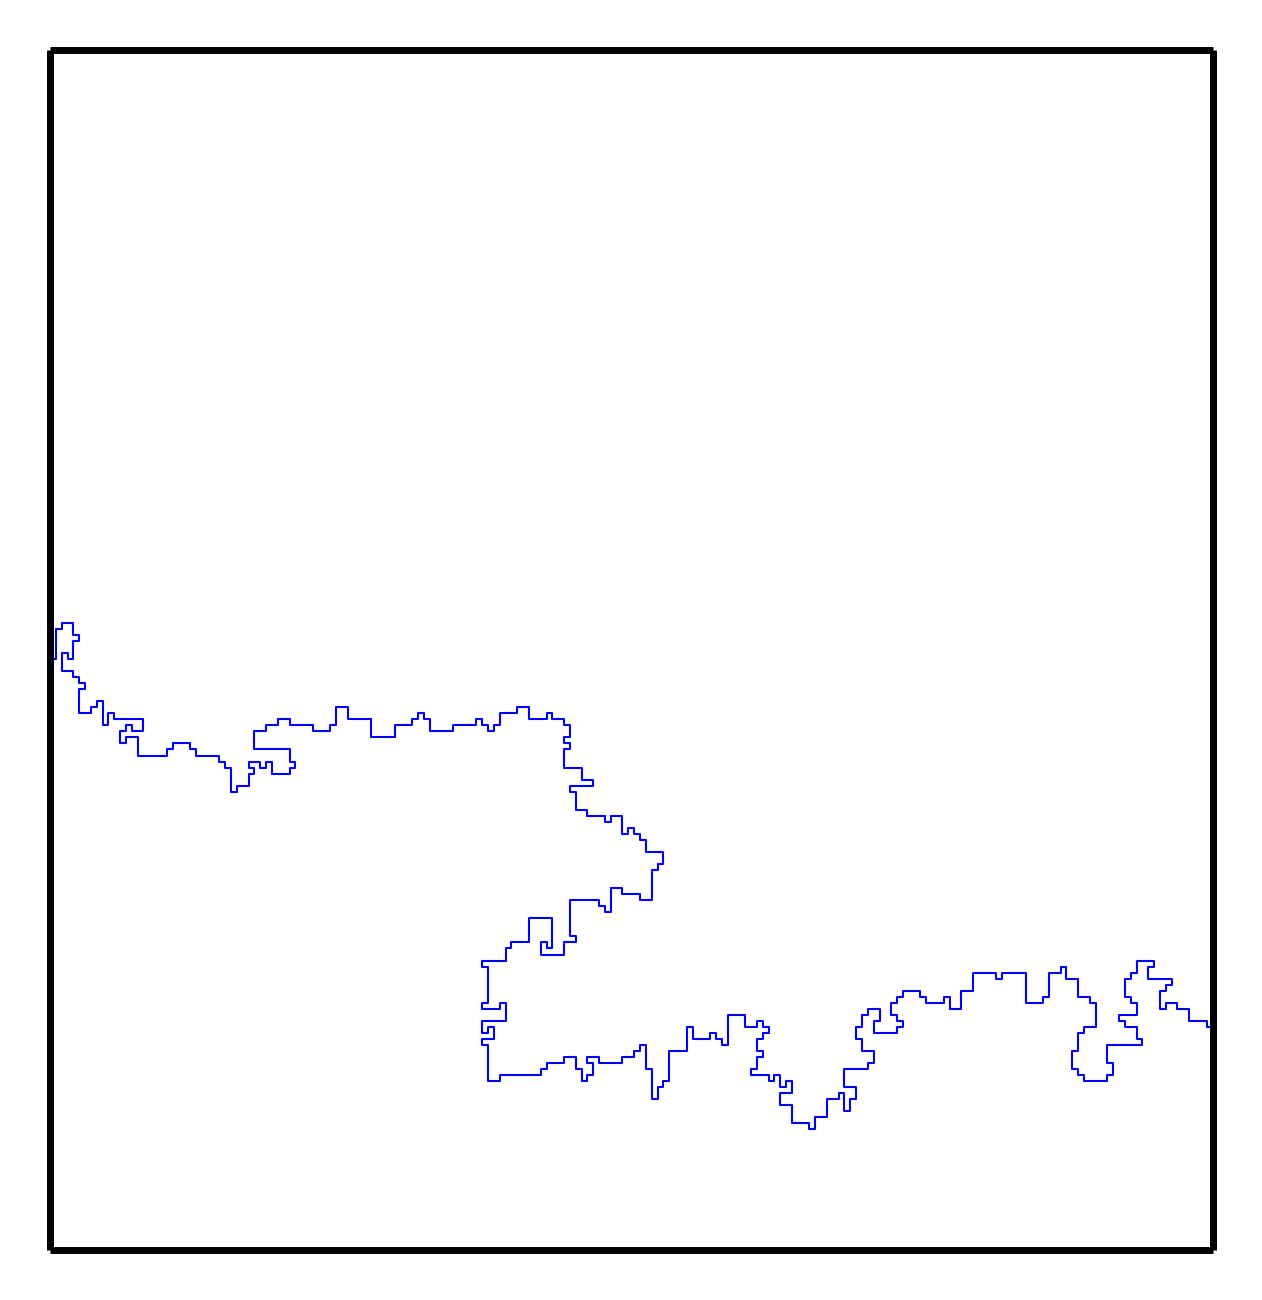
\includegraphics[scale=1.6]{LERW_200s7hdpi}
		\caption{Loop erased random walk on a $\mathbb{Z}^{\emph{2}}$ lattice (system size: 200; seed: 7)}
		\label{fig:LERW}
	\end{center}
\end{figure}

\subsection{Collecting Data}
	 All data collected for analysis was primary data generated by self-written code and systematic randomness. Data collection was an automatic procedure carried out by the code that I had written when run. A significant amount data had to collected for different system in order to draw a reliable and a more decisive conclusion. As discussed before, the main implication of the presence of periodic boundaries was that the size of the vertical component was indefinite and thus the size of the result was indefinite. Since the code could not be optimised for multithreading, the task for the execution of the code could not utilise more than one core of the multi-core computational infrastructure. Also considering that the computational infrastructure was not dedicated for the task (i.e other OS-related task have had a higher priority), it was apparent that the code had to run for a prolonged period of time in order to collect the necessary. Data was collected for different systems, namely, one dimensional random walk,
\newline
Fortunately, the computational resource available at disposal for this project were vast.  In particular, High Performance Computing (HPC). The source code was run on the HPC as a series of jobs over the period of a whole day (~24 hours) . Bash code was written to instruct the HPC to output the generated the data by the python interpreter as a series of UTF-8 encoded sequential .dat files (in the format required for analysis). Some metadata (such as the system size) was prepended to the files to distinguish and identify the files easier in analysis stage.
\newline
Data was collected for the following systems:
\begin{itemize}
	\item 2 dimensional Random Walks of system sizes of 50, 100, 200 and 400
	\item 1 dimensional Random Walks of system sizes of 50, 100, 200 and 400
	\item 2 dimensional Loop Erased Random Walks of system sizes of 50, 100, 200 and 400
\end{itemize}
On the first run on the cluster, we received a runtime error due to the incorrect configuration of the cluster but this was quickly fixed once the system was reconfigured. Once the files containing the data were generated, they were inspected manually to ensure that the generated data was valid (i.e. conformed to the expected data) and no logical errors where present in the code. Due to time constraints for each job of 15 hours on the cluster and considering that only one core of the cluster was being utilised, the code for generating the 2 dimensional Random Walks of system sizes of 400 and the code for generating 2 dimensional Loop Erased Random Walks of system sizes of 200, 400 was unable to completely execute. This incomplete execution resulted in the files not being generated (files were not completely written and so any associated temporary was discarded). Due to scarcity of time, I made the decision to just work with the data that we had obtained for the analysis instead of spending more time on generating data and produce less analysis. We agreed that this was the most productive course of action. Hence, \emph{in this report we will only analyse the data by a system\footnote{refer to \S~\ref{subsec:sysfdef} for definition} where} $|\vb{S}| \le 200$ .\newline

\section{Results and Analysis}
After the output .dat files were received, the data such as the return distributions needed to be plot as a histogram. The problem I encountered here was grouping the raw data in suitably sized bins in order to construct the histogram. Since the data was very large (up to 100MB), I we considered using a script written in \textit{C}. However, since this script was in \textit{C} and I was working in \textit{Python} so there was no programmatic way of exchanging the data (variables in one language could not be used in the other). Instead of rewriting this script in \textit{Python} and compromising performance, I figured out a way to exchange the data by modifying the script to output the data in a particular serialised format in \textit{C} and then parsing the output in \textit{Python} (refer to Appendix~\ref{sssec:histparse} for the code). Once parsed, the data was available in \textit{Python\'s} memory space and it could proceed to generate the histogram. The initial histogram depicted a very high positive skew as only a few significant values dominated resulting in an ambiguous trend. Discussing this, I found that this was due to great variation not being represented well due to the linear scales and so he advised me to use a double logarithmic scale.
	The double logarithmic histograms (refer to, Figure~\ref{fig:LERWhdish} -~\ref{fig:RW2Dhdish}) were used to qualitatively compare and evalulate the return times distributions for 2 dimensional discrete ($\mathbb{Z}^{\emph{2}}$) LERWs, 2 dimensional discrete ($\mathbb{Z}^{\emph{2}}$) Random Walks and 1 dimensional discrete ($\mathbb{Z}$) Random Walks. \newline

What my research found was that was that return times distribution for $\mathbb{Z}^{\emph{2}}$ random walk and return times distribution for $\mathbb{Z}$ random walk were very similar. What my research also found that there is a difference in the distribution of the return times of a random walker (1D and 2D) and the distribution of the loops erased in LERW.

\paragraph{Return distribution of 1D and 2D Random Walks.} Comparing Figure~\ref{fig:RW1Dhdish} and Figure~\ref{fig:RW2Dhdish}), I found that the return times distribution for $\mathbb{Z}^{\emph{2}}$ random walk and return times distribution for $\mathbb{Z}$ random walk were very similar. For a random walk in one dimension starting at $n$, the probability that the random walk eventually returns to $n$ equals one \cite{Redner2002} $\implies \Pr(S_{n}=n) = 1$, $n \in \mathbb{Z}$. However, the time required to return to $n$, averaged over all possible vertices in the system, is infinite.  We conclude that this observation is due to the survival probability $S(t)$ ultimately decaying to zero for a random walk in two dimensions. This means that a random walk is recurrent - it is certain to eventually return to its starting point, and indeed visit any vertex of an infinite lattice. This is the $2.$ deduced characteristic stated in $\S1.1$. This is also because of the fact that a random walk has no memory (random variables independently distributed) and so it transits to a new state (i.e. resets it\' s state) every time a specific lattice vertex is transversed. Hence, recurrence also implies that every site is visited infinitely often.

The arcsin law, which is concerned with the statistics of returns to the origin, also applies here as our random walk is an unrestricted random walk. From the arcsine law, we can infer that the most probable outcome is that the walk always remains entirely on the positive or on the negative axis. This is against the natural expectation of approximately one-half of the total time being spent on the positive axis and the remaining one-half of the time on the negative axis for a random walk which starts at x = 0. Surprisingly, the natural expectation is the least probable outcome.\newline
\paragraph{Difference in arc length distribution of returns and loops erased.} As depicted in Figure~\ref{fig:AREr}, there is a correlation between the distribution of the loops erased in a random walk and the probability of return to (an arbitrary) vertex in the lattice for both systems of size 100 and 200. In fact, the combined distribution is positively skewed which implies that as the loops erased increase, the probability of returning to a vertex in the lattice decreases. The fact that the data is skewed, indicates that there is a difference arc length distribution of a random walker returning and arc length distribution of the loops erased.

\begin{figure}[H]
	\centering
		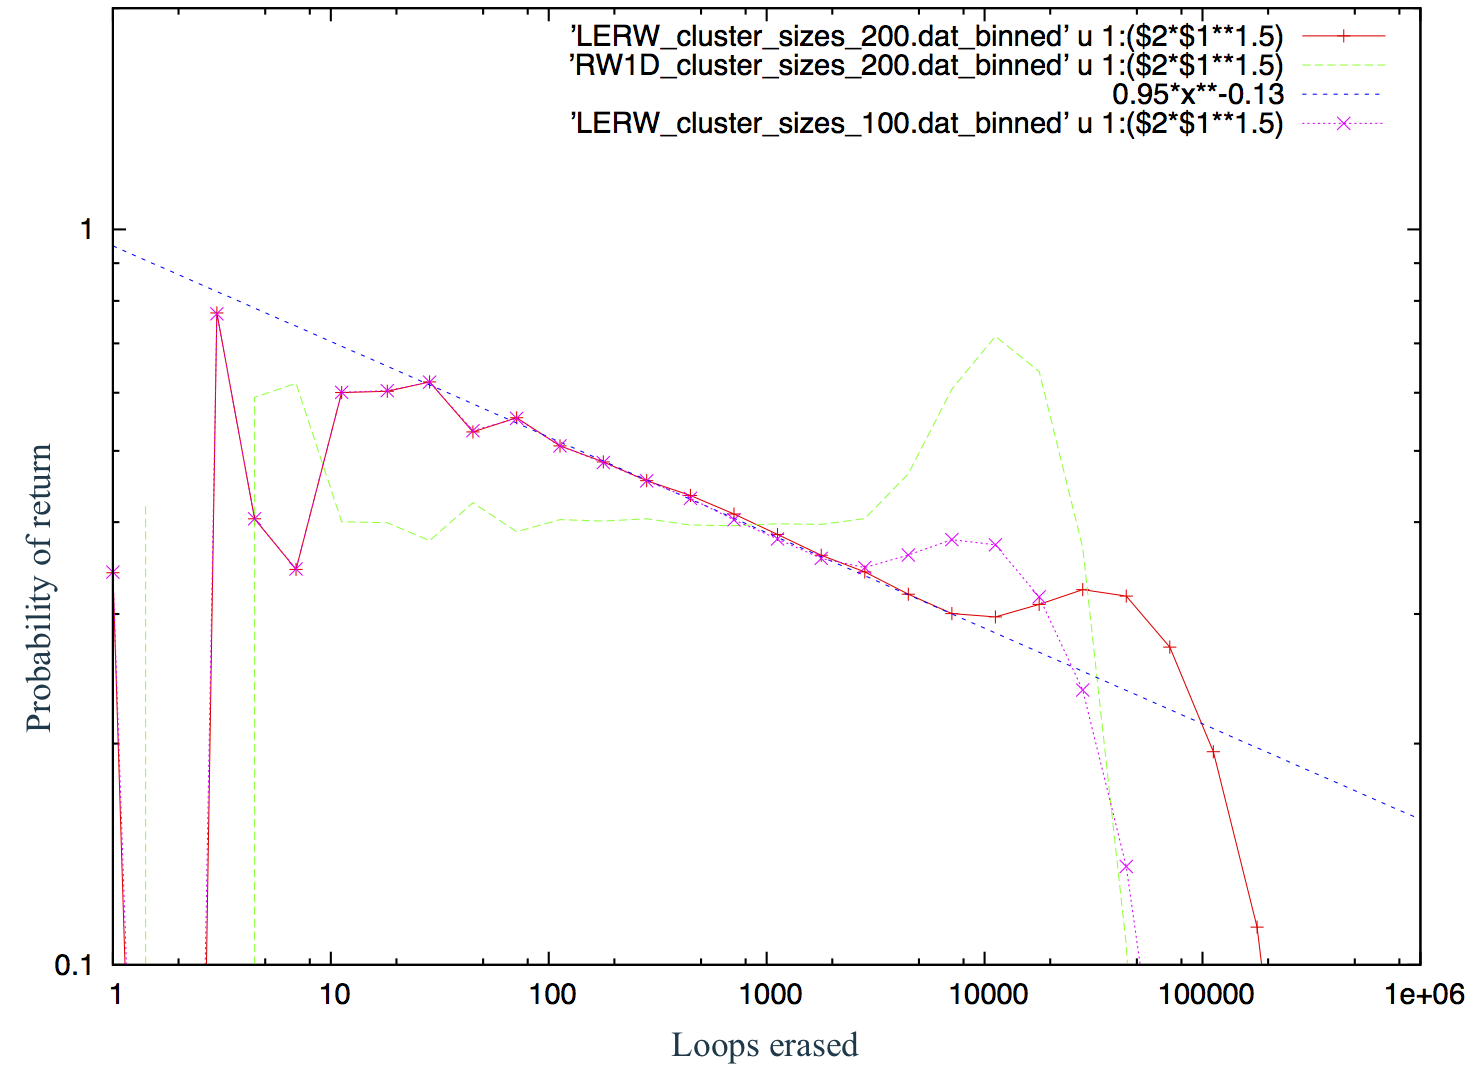
\includegraphics[scale=0.6]{preturn_le_plot}
		\caption{Probability of return and loops erased distributions for $\mathbb{Z}^{\emph{2}}$ LERWs (system sizes: 100, 200; seed:10) and $\mathbb{Z}$ Random Walk (system size:200; seed:10)}
		\label{fig:AREr}
\end{figure}
\begin{figure}[H]
	\centering
		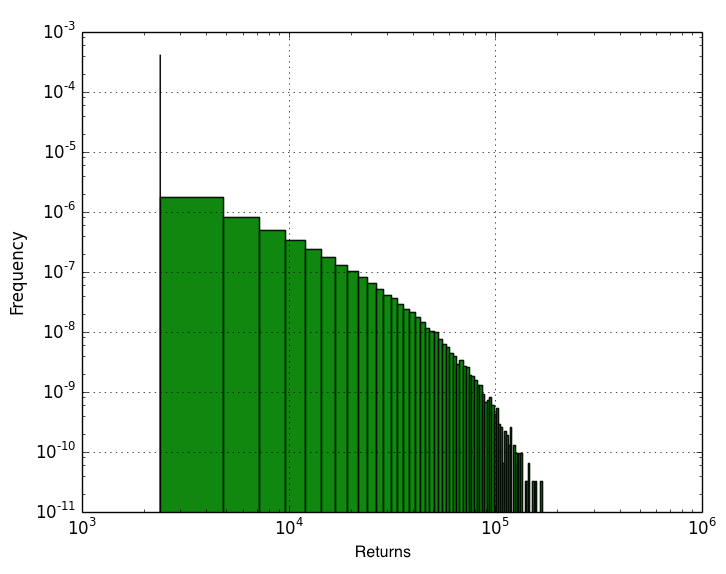
\includegraphics[scale=0.5]{LERW_cluster_sizes_200_histogram}
		\caption{Histogram for the distribution of the Loop Erased for Random Walks on $\mathbb{Z}^{\emph{2}}$ lattice (system size:200; seed:10)}
		\label{fig:LERWhdish}
\end{figure}
\begin{figure}[H]
	\centering
		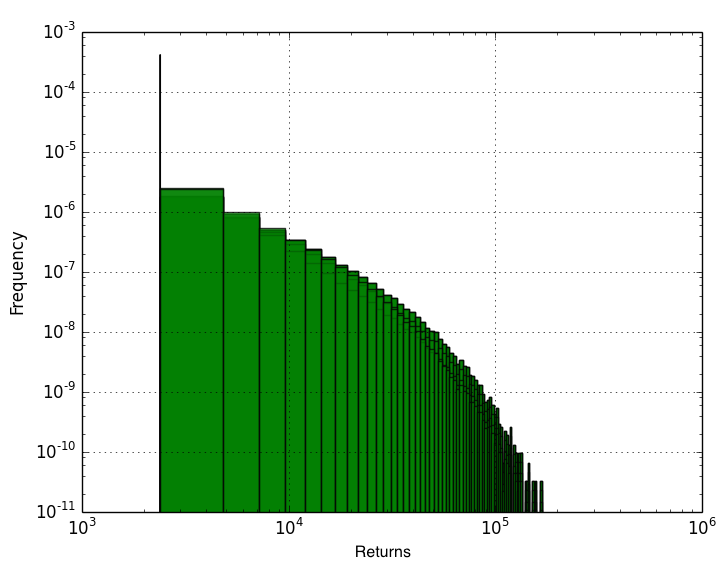
\includegraphics[scale=0.5]{RW1D_cluster_sizes_200_histogram}
		\caption{Histogram for the returns distribution of Random Walks on $\mathbb{Z}$ lattice (system size:200; seed:10)}
		\label{fig:RW1Dhdish}
\end{figure}
\begin{figure}[h]
	\centering
		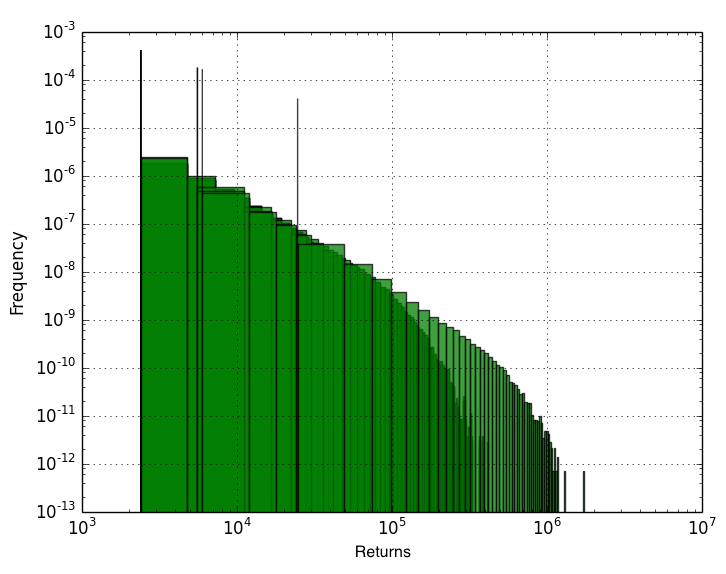
\includegraphics[scale=0.5]{RW2D_cluster_sizes_200_histogram}
		\caption{Histogram for the returns distribution of Random Walks on $\mathbb{Z}^{\emph{2}}$ lattice (system size; seed:10)}
		\label{fig:RW2Dhdish}
\end{figure}
\newpage

\section{Conclusion}
\subsection{Findings}
The research has shown that the return distribution of a one-dimensional random walk and a two-dimensional random walk is almost identical. It can be concluded that the similarity in the return distribution of the one-dimensional random walk and the two-dimensional random walk is due to the survival probability of the two-dimensional random walk eventually being zero. Since the return probability of a one-dimensional random walk is one, this means that return probability of a two-dimensional random walk is very close to one. We can also conclude that there is a difference in the distribution of the return times of a random walker and the distribution of the loops erased in LERW.

To further develop this research, I would incorporate the usage of Self Avoiding Random Walks (SARW) which are random walks that do not self-intersect during their transversal and are in a different universality class from LERW. I would also consider the relationships in the statistics of enclosed area between bidirectional LERWs, the statistics of the intersections and the variance of the number of intersections. A more abstract area that could be explored is the topography of LERWs, in particular, the average eccentricity of the loop erased random walk trajectory.

\subsection{Implications}
I believe that the results that I have obtained could have an impact on many stochastic processes and on the people whose careers are associated with them. The return probability of a two-dimensional and a one-dimensional random walk being almost identical implies that a stochastic process modelled using two essential (independent) random variables will inevitable return to its current position. What this means in the real world, for instance in stock market is that the price of a stock on the stock market with respect to time (where the stock price and time are the two random variables) will eventually return to its current stock price (over an indefinite time period). In this application case, this discovery may be beneficial to shareholders as it allows them to anticipate a future market position and make actionable decision with that information. The cumulative effect of this could dictate the the future of the market both short-term and long-term. Similarly, when applied in a network, this discovery asserts that the current bandwidth usage in network will eventually be reached again over an indefinite time period. This could prompt network administrators to anticipate peak bandwidth usage by deducing the return to peak bandwidth usage time and allocate the resources across the network more efficiently.

\appendix
\section{Appendices}
	\emph{Please note that any variables/constants declared are accessible throughout (globally) the (8.x) code sections respectively of their scope. Also note that this is not all the code produced for the research project but only parts that this report explores. Appendix ~\ref{sssec:imports} declares the libraries used globally and their respective identifiers used to reference them in the subsequent code.}
	\subsection{Imports} \label{sssec:imports}
	\lstinputlisting[language=Python]{pysc/import.py}
	\subsection{System Definition code} \label{sssec:sysdef}
	\lstinputlisting[language=Python]{pysc/sysdef.py}
	\subsection{Random Walk generation code} \label{sssec:srwgen}
	\lstinputlisting[language=Python]{pysc/srwgen.py}
	\subsection{Loop Erased Random Walk code} \label{sssec:lerw}
	\lstinputlisting[language=Python]{pysc/lerw.py}
	\subsection{Random Walk plot code (using the matplotlib API)} \label{sssec:rwplot}
	\lstinputlisting[language=Python]{pysc/plot.py}
	\subsection{Loop Erased Random Walk plot code} \label{sssec:lerwplot}
	\lstinputlisting[language=Python]{pysc/lerwplot.py}
	\subsection{Histogram plot (and parse from raw2bin.c) code} \label{sssec:histparse}
	\lstinputlisting[language=Python]{pysc/histparse.py}
\hphantom
\newline
\section{Bibliography}
	\bibliographystyle{amsplain}
	\bibliography{references}
\hphantom
\newline
\section{Acknowledgements}
I would like to thank Professor Gunnar Pruessner of Imperial College London for supervising the research project and the Nuffield Foundation for funding this research. I would also like to thank Imperial College London for allowing us to use the High Performance Computing (HPC) mainframes at Huxley Building in ICL.

\hphantom
\newline
\textless\textgreater\ $with$ \textless3 $by$ Habib Rehman

\end{document}
